\section{Aplicações}

O \textsc{Subset-Sum} é um problema muito parecido com o Problema da Mochila (\textsc{Knapsack}) que é um \textbf{problema de otimização} enunciado como: dado um conjunto de $n$ itens $i$, cada um com uma massa $w_i$ e um valor $v_i$, determine quais itens pegar de modo que o total de peso seja menor ou igual a um limite $W$ e o total de valor seja maior ou igual a $K$, desde que não ultrapasse o limite $W$.

Portanto, o \textsc{Subset-Sum} é um caso especial do \textsc{Knapsack}, onde $s_i = v_i = w_i$, $t = K = W$, e logo serve como base para seu entendimento -- inclusive, poderia ser feita a redução \textsc{Knapsack} $\rightarrow$ \textsc{Subset-Sum} para provar sua \textbf{NP}-\textit{completude}. Por sua vez, o \textsc{Knapsack} pode ser aplicado no mundo real para otimização no carregamento de cargas para transporte, empacotamento de produtos, orçamentos e investimentos de capital.

% inkscape -D -z --file=./input/smooth.svg --export-pdf=./input/smooth.pdf

% \begin{figure}[h]
%	\centering
%	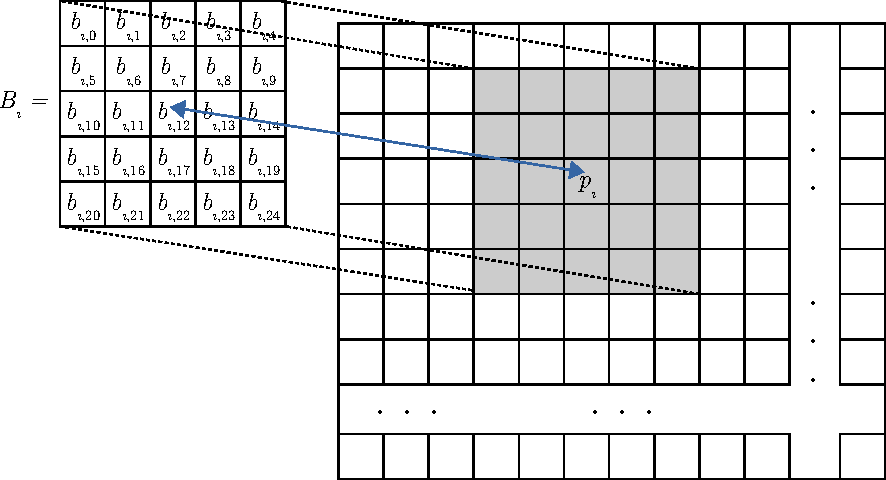
\includegraphics[scale=1]{./input/smooth.pdf}
%	\caption{Ilustração da aplicação de \textit{smooth} em um pixel $p_i$ de uma imagem. \label{fig:ilustracao}}
% \end{figure}

